\section{Proactive BPSP}
\label{sec:method}

\begin{figure*}[t]
\centering
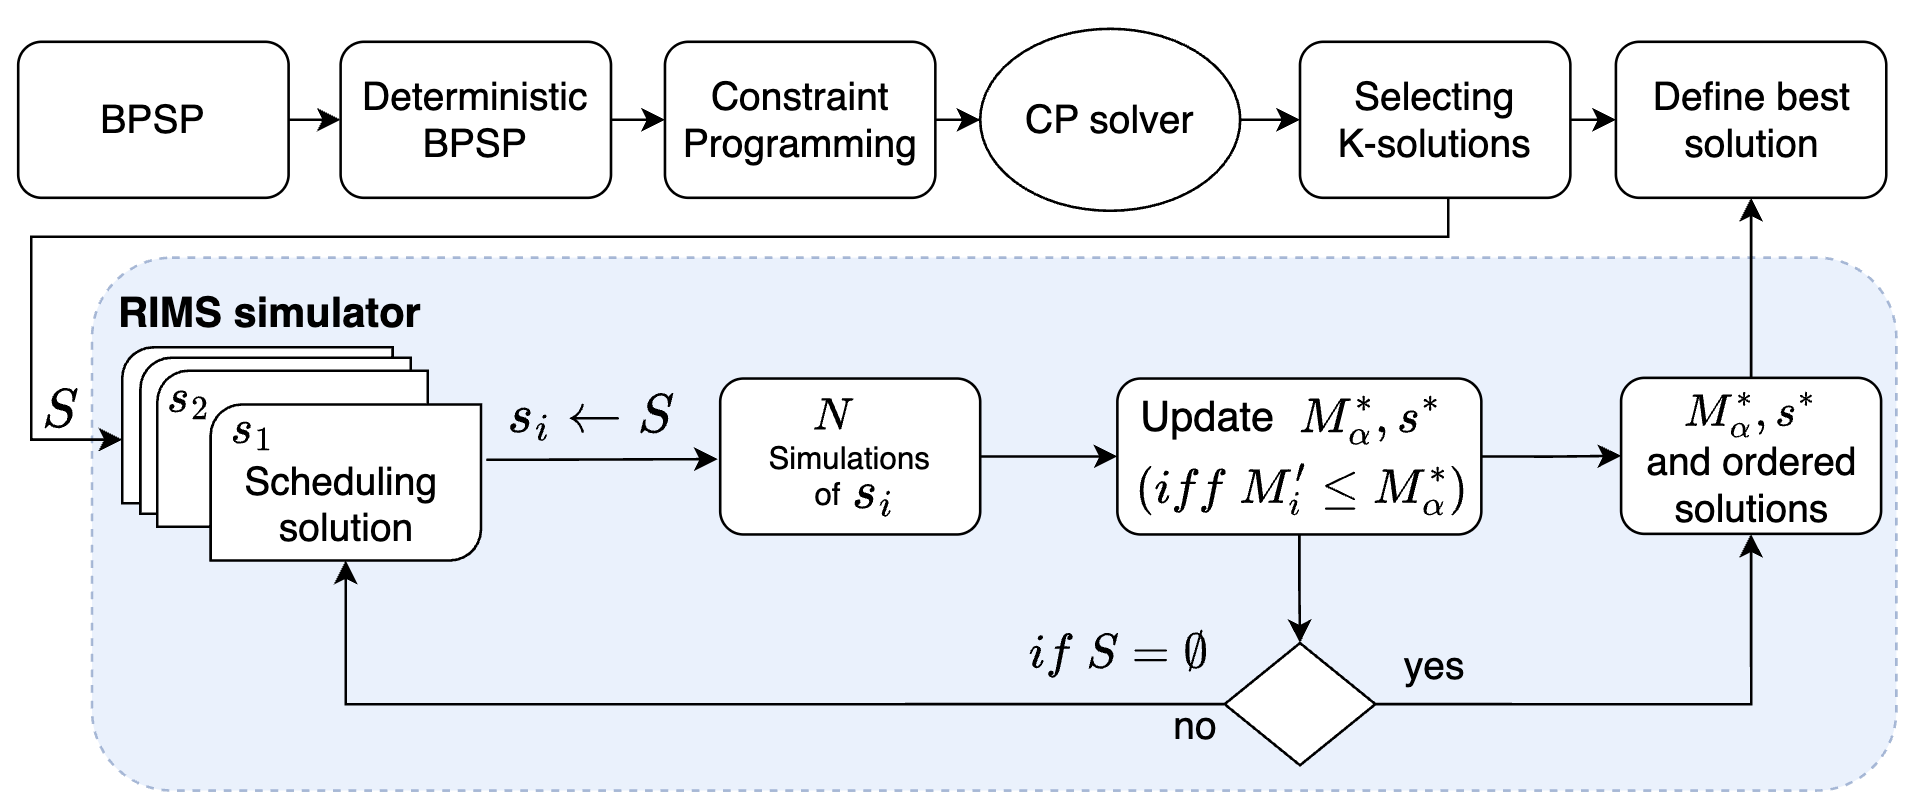
\includegraphics[width=0.6\textwidth]{images/pipeline_rims3.png}
\caption{Our approach to Proactive Business Process Scheduling.}
\label{fig:pipeline}
\end{figure*}
Figure~\ref{fig:pipeline} illustrates the steps of our method. First, we define the BPSP based on either prior knowledge or by estimating its parameters from data.
To manage the stochastic activity durations, we convert the stochastic BPSP into its deterministic counterpart by employing the transformation proposed in~\cite{beck2007proactive}, which is described in the next Section.
Next, once the problem becomes deterministic, we construct a Constraint Programming (CP) model, and a CP solver is employed to obtain solutions that iteratively minimize the global Makespan $M$ until either an optimal deterministic solution is found, or a time limit is reached. Once CP solutions are obtained, we first select the \emph{top-$K$} solutions. Finally we employ Monte-Carlo simulation to identify the best solution. Below, we detail the different steps, and justify our design choices.


\subsection{From Stochastic to Deterministic BPSP}
\label{sec:stoc_to_det}

The activity durations in a BPSP are random. Therefore, minimizing 
the Makespan
implies
finding the smallest possible value of $M^*_\alpha$ such that a solution exists with a random Makespan that, with high probability, $1-\alpha$ is less than $M^*_\alpha$. We refer to $M^*_\alpha$ as the probabilistically minimum Makespan.

To transform the BPSP into a deterministic problem, we use the approach proposed by~\cite{beck2007proactive}, which associates a deterministic problem with the probabilistic one by transforming each random duration into the sum of its mean value and a buffer that depends on its standard deviation. More formally, for activity $a_j$ in case $i$, the deterministic duration
that is associated with it is, \begin{equation}
d_{i,a_j} = \mu_{i, a_j} + q \cdot \sigma_{i, a_j},\label{eq:duration}
\end{equation} with 
$\mu_{i, a_j}$ being the mean duration
of the activity, $\sigma_{i, a_j}$ being its standard deviation
and $q\geq0$ being
an uncertainty coefficient that provides a buffer for the mean value.\footnote{Note that we assume the existence of the first two moments of the distribution for activity durations.}
If $q=0$, the mean value is used as activity duration across the board.
All other components of the problem are deterministic, 
and remain unchanged. 
%The approach is grounded in theory, which we lay out, and extend in the following part.
The challenge with the transformation defined in \eqref{eq:duration} is the identification of the value of a value of $q$ such that the makespan $M_q$ of the deterministic problem serves as a lower bound for the makespan $M_\alpha$ of the stochastic problem. In the remaining of the Section we provide some details on the solution proposed in~\cite{beck2007proactive} and summarized the value of $q$ defined in \eqref{eq:qU}.


\subsubsection{Lower-Bound Guarantees for BPSP} 


The work in~\cite{beck2007proactive} shows that for Resource-Constrained Project Scheduling Problem (RCPSP),
a lower bound for the probabilistic Makespan $M^*_\alpha$ is provided by the makespan $M_U$ given by the solution of the deterministic problem obtained using the transformation \eqref{eq:duration} with the value of  $q$ set to
\begin{equation}
q_U = \frac{\Phi^{-1}(1-\alpha)}{\sqrt{U}},
\label{eq:qU}
\end{equation}
where $\Phi^{-1}$ is the inverse of the standard normal cumulative distribution function (CDF), and $U$ represents an upper bound on the number of uncertain activities along the deterministic critical path (e.g., $U$ can be set to the total number of activities).
Furthermore, the authors in~\cite{beck2007proactive} demonstrate that this lower bound can be tightened by selecting different values for \( q \) when additional assumptions are satisfied. The lower bound result is critical to efficiently select models using Monte Carlo simulation.


However, to apply the result in the BPSP case, we must overcome three violations of the classical RCPSP assumptions, namely multiple cases, potentially inter-dependent activity durations, and planned resource unavailability. 
The first two violations are straightforward to address.  
Since we consider the Makespan with respect to the latest activity regardless of the case, one can view BPSP as a single-case scheduling problem~\cite{sanchez2023survey}.  
Moreover, when conditioning on the case, the resources, and the activity being processed, activity durations become independent of each other. This property, referred to as conditional independence, ensures that the result from~\cite{beck2007proactive} applies, as we assume the case identifier and activity information (i.e., its type and required resource set) are known.  

The only significant limitation that remains unresolved relates to resource calendars.
To prove that $q_U$ indeed yields a lower-bound we must
first define so-called \emph{positive precedence expressions}.
The set $E$ is a set of precedence constraints between activities $a_i$ and $a_j$ specified as $\texttt{before}(i, j)$, i.e., the constraint that activity $a_j$ cannot 
start earlier than the completion of $a_i$.
%For activities $a_i$ and $a_j$, the expression $\texttt{before}(i, j)$ represents the constraint that activity $a_j$ cannot start earlier than the completion of $a_i$. 
We are now ready to define positive precedence expressions (PPEs). 

\begin{definition}[Positive Precedence Expressions (PPE)]
\label{def:ppe} 
The set $E$ is referred to as a positive precedence expressions over a set of activities $A$ if it is the smallest set satisfying:
\begin{enumerate}
    \item $ \forall a_i, a_j, \texttt{before}(i, j) \in E$.
    \item If $\phi, \psi \in E$, then $\phi \wedge \psi \in E$ and $\phi \vee \psi \in E$.
\end{enumerate}
\end{definition} In~\cite{beck2007proactive} it is 
shown that for scheduling problems that 
can be written as a conjunction of PPEs,
the proposed transformation that uses $q_U$ (as above) provides a lower-bound
on the stochastic problem. Therefore,
what remains to be shown is that BPSP can be expressed 
by a conjunction of PPEs.
\begin{proposition}
Selecting $q= q_U$ yields a lower-bound solution to the stochastic BPSP. \label{prop:lower}
\end{proposition}
\begin{proof}
We build the proof on the result of~\cite{beck2007proactive}, who established a lower bound for RCPSPs that do not account for resource unavailability. We will treat resource `vacations'
as dummy activities that we must schedule in addition to the other activities. The core argument relies on the ability to represent RCPSP constraints as Positive Precedence Expressions (PPEs).
Specifically, the constraints of an RCPSP can be expressed as a conjunction of PPEs~(\cite{beck2007proactive}):
\begin{enumerate}
    \item \textbf{Precedence Constraints (\( \phi \))}: Precedence relationships between activities \( a_i \) and \( a_j \) are represented as primitive precedence expressions \( \texttt{before}(i, j) \). Let \( \phi \) denote the conjunction of all such precedence constraints.

    \item \textbf{Resource Constraints (\( \psi \))}: Resource constraints can be represented using forbidden sets. A forbidden set \( H \subseteq \mathcal{A} \) consists of activities whose simultaneous execution exceeds the capacity of a resource \( r \), $C_r$. Resource constraints are satisfied if, for all \( H \in F \), there exist two activities \( a_i, a_j \in H \) such that \( \texttt{before}(i, j) \) holds. This is expressed as:
    \[
    \psi = \bigwedge_{H \in F} \bigvee_{a_i, a_j \in H, i \neq j} \texttt{before}(i, j).
    \]
\end{enumerate} Combining these, the constraints of an RCPSP are represented as \( \phi \wedge \psi \), which is a conjunction of PPEs. In BPSP, resource unavailability introduces additional constraints:
each resource \( r \) has an availability calendar \( v_{r,t} \), where \( v_{r,t} = 1 \) if \( r \) is available at time \( t \), and \( 0 \) otherwise.
To incorporate resource unavailability, we redefine and extend the notion of forbidden sets:
\begin{enumerate}
    \item Capacity forbidden sets \( H \) are defined as in RCPSPs, representing sets of activities whose simultaneous execution exceeds the capacity of a resource \( r \).
    \item For resource unavailability, we extend \(H\) with additional constraints for each resource \( r \) and time \( t \) where \( v_{r,t} = 0 \). The extended forbidden sets, denoted $H'$, ensure that no activities requiring \( r \) overlap during unavailable periods.
\end{enumerate} The resource constraints with unavailability can then be expressed as:
\[
\psi_u = \bigwedge_{H' \in F'} \bigvee_{a_i, a_j \in H', i \neq j} \texttt{before}(i, j),
\]
where \( F' \) is the extended set of forbidden sets that includes both capacity constraints and unavailability constraints.

The combined constraints for BPSP, including resource unavailability, can now be expressed as:
\[
\phi \wedge \psi_u,
\]
where \( \phi \) represents precedence constraints, and \( \psi_u \) represents resource constraints, including unavailability. Each component is a conjunction of PPEs, ensuring that the overall problem retains the PPE structure.

Since BPSP constraints can be expressed as a conjunction of PPEs, the results from~\cite{beck2007proactive} apply, and \( q_U \) provides a lower bound on the stochastic Makespan.

\end{proof} 


% \begin{proofsketch}
% This proof builds on~\cite{beck2007proactive}, who showed that Resource-Constrained Project Scheduling Problem (RCPSP) constraints can be expressed as a conjunction of Positive Precedence Expressions (PPEs). Precedence constraints (\( \phi \)) are primitive expressions \( \texttt{before}(i, j) \), and resource constraints (\( \psi \)) are modeled using forbidden sets, ensuring no subset of activities requiring the same resource exceeds its capacity. Together, RCPSP constraints form \( \phi \wedge \psi \), retaining the PPE structure.


% To handle resource unavailability in the BPSP, forbidden sets are extended. For each resource \( r \) and time \( t \) where \( v_{r,t} = 0 \), additional constraints ensure that activities requiring \( r \) do not overlap during unavailable periods. These extended forbidden sets, \( H' \), combine capacity and unavailability constraints, forming \( \psi_u \). The BPSP constraints are then expressed as \( \phi \wedge \psi_u \), preserving the PPE structure. \btext{In essence, unavailability periods are injected as `dummy' activities that must be considered when scheduling.} 

% Since BPSP constraints remain a conjunction of PPEs, the results reported in~\cite{beck2007proactive} apply directly. Thus, \( q_U \), a lower bound for RCPSPs, extends as a valid lower bound on the stochastic Makespan of BPSPs, even with resource unavailability.\footnote{Full proof is available in the supplementary material.}
% \end{proofsketch}

%We shall use this result in the 
%last part of our approach where we select 
%stochastic candidates based on deterministic solutions and Monte-Carlo %simulation.



%\textit{Evaluating a solution of a probabilistic RCMSPS can be done by using Monte Carlo Simulation: for each of a large number of trials we randomly sample the durations of every activity and generate the makespan associated with that trial}. We fix $\alpha$ to bound the probabilities and we assume a value in range $(0, 0.05]$.

\subsection{Solving Deterministic BPSP with CP}

%We use a common formalism to model RCPSP problems that involve optional activities and alternative resources~\cite{baptiste2001constraint,liu2019robust,ari}, and .
In this section, we present a CP model of the 
deterministic BPSP. We use the general CP model
proposed by \cite{senderovich2019learning}, 
and extend it with the planned unavailability~\cite{hauder2020resource}.

In particular, we employ the optional interval variable, $var$, to effectively represent the activities in our deterministic BPSP. The presence, start time, and duration are represented by \act{Pres}($var$), \act{Start}($var$) and 
\act{Length}($var$), respectively, with \act{Pres}($var$)~$=0$ indicating
its absence in the constraint model.
For each activity, $a_j \in A_i$, to be executed in a case $i$ we define an interval variable $x_{i,a_{j}}$ where~\act{Start}($x_{i,a_{j}}$)~$\geq 0$ and~\act{Pres}($x_{i,a_{j}}$)~$= 1$. The precedence relations between the activities in $i$ are guaranteed by the form \act{EndBeforeStart}~($x_{i,a_{k}},x_{i,a_{j}})$ $ \forall a_k \in \Pi_{i,a_j}$, ensuring that \act{Start}($x_{i,a_{j}}$) $\geq$ \act{Start}($x_{i,a_{k}}$) $+$ \act{Length}($x_{i,a_{k}}$). %Each activity can be performed by exactly one resource respecting its planned unavailability. 
To represent the resources assignments we define, $$X_{a_j}~=\{\overline{x}_{i,a_j,R}: d_{i,a_j},R \subseteq \mathcal{R}\},$$ as set of optional interval variables, where $\overline{x}_{i,a_j,R}$ represents the activity $a_{j} \in A_i$ assigned to a set of resources $R \subseteq \mathcal{R}$ with duration \act{Length}($\overline{x}_{i,a_j,R}$)$= d_{i,a_j}$ defined as~\eqref{eq:duration}.

%where $\overline{x}_{i,a_j,r}$ represents the activity $a_{j} \in A_i$ assigned to resource $r \in \mathcal{R}$ with duration \act{Length}($\overline{x}_{i,a_j,r}$)$= d_{i,a_j}$ defined as~\eqref{eq:duration}. 

\act{Alternative}(${x}_{i,a_j}, X_{a_j}$) ensures that only one interval variable from $X_{a_j}$ is present, and it starts and ends together with ${x}_{i,a_j}$. \act{Unavailable}($\overline{x}_{i,a_j,r}, v_{r,t}$) guarantees that the start and end times of the activity overlap with an available period in the resource calendar, $v_{r,t}$.
Finally, to ensure that the total number of present and executing activity interval variables assigned to a resource does not exceed its capacity, we define \act{Cumulative}($\{\overline{x}_{i,a_j,r}: a_j \in A_i \}, C_r$), $\forall r \in \mathcal{R} \; \text{and} \; \forall i \in \mathcal{I}$.

The goal is to minimize the global Makespan, i.e., the maximum end time across all activities.
\[
\text{Makespan} = \max_{i \in \mathcal{I}, a_j \in A_i} \text{\act{Start}}(x_{i,a_j}) + \act{Length}(x_{i,a_j})
\]




\subsection{Solution Selection \& Monte Carlo Simulation}

In this phase, we apply a CP solver\footnote{We use the Python version of Google OR-Tools (v9.11.4210) as our CP solver.} to
collect feasible solutions that iteratively minimize 
the global Makespan until either the optimal solution is found or a pre-defined time limit is reached. 
To evaluate the solutions returned by the CP solver and we employ Monte Carlo Simulation to select, $M_\alpha^*$, the one that yields the probabilistic minimum Makespan. 
%-- i.e., a solution that, with high probability $1 -\alpha$ guarantees a Makespan lower than $M^*_{\alpha}$ -- we employ Monte Carlo simulation. 
$M_\alpha^*$ is defined as the 
$
M_\alpha^* = \min_{s_i \in S} M'_{s_i}
$
where $M'_{s_i}$ represents the $100(1 - \alpha)$th percentile of Makespan
values computed over $N$ Monte Carlo simulations of a solution $s_i$ returned by the CP solver.
Each Makespan value, corresponds to the maximum end time across all activities in the simulation

Firstly, we select a subset of $k$-solutions from those returned by the solver, leveraging the 
well-established correlation between deterministic and probabilistic solutions~\cite{BonfiettiLM14}.\footnote{The evaluation section provides a detailed explanation of the $k$-solutions selection process.} 
Then, we iteratively evaluate selected solutions by performing a large number of independent simulations using the original stochastic activity durations to identify $M^*_{\alpha}$.  

